% !TEX root = ../main.tex

\chapter{Konzept \& Design}
\label{ch:KuD}

Nachdem in den vorherigen Kapiteln die Grundlagen gelegt und die Lücken der bestehenden Systeme analysiert wurden, wird nun der Entwurf der Lösung thematisiert. In diesem Kapitel wird der Entwurf des Frameworks zur automatisierten Architekturvalidierung von Anforderung bis zum detaillierten Design nachvollziehbar dargelegt. Im ersten Abschnitt werden daher die Spezifikationen der funktionalen und nicht-funktionalen Anforderungen präsentiert. Auf dieser Basis wird anschließend der Architekturentwurf vorgestellt, welcher die Einbettung in das übergeordnete System erläutert. Die nachfolgenden Abschnitte fokussieren diesen Entwurf durch das detaillierte Konzept der \gls{api}, der Algorithmus-Ausführung, dem ersten Validierungsalgorithmus sowie dem Design der \gls{gui}.


\section{Anforderungsanalyse}
\label{sec:Anforderungsanalyse}

Eine präzise Definition der Anforderungen ist die zwingende Voraussetzung für eine zielgerichtete Entwicklung. Basierend auf der Analyse der bestehenden Systemlücke werden daher die funktionalen und nicht-funktionalen Anforderungen an das zu entwickelnde Framework in Tabelle~\ref{tab:anforderungen} spezifiziert. Diese bilden die verbindliche Grundlage für alle nachfolgenden Design- und Implementierungsentscheidungen.

\begin{table}[ht!]
  \centering
  \footnotesize
  \begin{tabularx}{\textwidth}{l l X}
    \toprule
    \textbf{ID} & \textbf{Anforderung}           & \textbf{Beschreibung}                                                                                                                                                                   \\
    \midrule
    \multicolumn{3}{c}{\textit{Funktional}}                                                                                                                                                                                                \\
    \midrule
    FA-1        & Algorithmen-API                & Bereitstellung einer API, die es Nutzern ermöglicht, Validierungsalgorithmen zu verwalten (hochladen, bearbeiten, löschen) und auszuführen.                                             \\
    \midrule
    FA-2        & Algorithmenverwaltung-GUI      & Bereitstellung einer \gls{gui} zur Verwaltung von Validierungsalgorithmen. Diese muss Funktionen zum Hochladen, Bearbeiten, Löschen sowie zum Starten der Ausführung umfassen.          \\
    \midrule
    FA-3        & Ergebniss-GUI                  & Bereitstellung einer \gls{gui} zur visuellen Darstellung der Ergebnisse von Validierungsläufen. Die \gls{gui} muss verschiedene Ausgabeformate (z. B. textuell, grafisch) unterstützen. \\
    \midrule
    FA-4        & Erster Validierungsalgorithmus & Bereitstellung eines ersten Validierungsalgorithmus, der eine grundlegende Architekturprüfung durchführt.                                                                               \\
    \bottomrule
    \multicolumn{3}{c}{\textit{Nicht-Funktional}}                                                                                                                                                                                          \\
    \midrule
    NFA-1       & Standardisierte API            & Die zu entwickelnde API muss den Prinzipien des \gls{rest}folgen.                                                                                                                       \\
    \midrule
    NFA-2       & Benutzerfreundlichkeit         & Die GUI muss intuitiv bedienbar sein.                                                                                                                                                   \\
    \bottomrule
  \end{tabularx}
  \caption{Anforderungen an das Framework}
  \label{tab:anforderungen}
\end{table}

Im Folgenden wird die Notwendigkeit für jede dieser Anforderungen näher erläutert.

\subsection*{Algorithmen-\gls{api}}

Ein zentrales Element des Frameworks ist die Bereitstellung der \gls{api}, um die Validierungsalgorithmen an das ArchitekturTool binden zu können (FA-1). Diese Funktion ist die Grundvoraussetzung, um das System, wie im Ziel der Arbeit gefordert, erweiterbar zu gestalten. Um die Integration weiterer bzw. Anpassung bestehender Funktionalitäten für Entwickler zu vereinfachen und eine hohe Kompatibilität zu gewährleisten, wird zudem die Einhaltung des \gls{rest}-Standards gefordert (NFA-1). Dieser etablierte Standard fördert eine lose Kopplung zwischen Framework und den angebundenen Algorithmen und ermöglicht eine schnelle Einarbeitung für Entwickler, die nicht vertraut sind mit dem Programm.

\subsection*{Grafische Benutzeroberfläche}

Für die Interaktion mit dem Nutzer ist eine \gls{gui} zur Verwaltung der Algorithmen essenziell (FA-2). Sie muss alle notwendigen Funktionen wie das Hochladen und Ausführen der Validierungsalgorithmen ermöglichen. Um einen reibungslosen Ablauf beim benutzen des Tools zu gewährleisten, muss die Bedienung intuitiv und selbterklärend sein (NFA-2). Die Benutzerfreundlichkeit ist entscheidend für die Ingenieure und Entwickler im Arbteitsalltag. Des Weiteren müssen die Ergebnisse der Architekturvaliderungen visuell aufbereitet und ausgegeben werden (FA-3). Ohne eine Visualisierung der Ergebnisse ist es für den Nutzer schwer ersichtlich, was genau die Validierung ergeben hat. Die Unterstützung verschiedener Visualisierungsarten, wie textueller oder grafischer Ausgaben, ermöglichen es dem Nutzer, die Fehlerursache bzw. den Engpass effizient zu identifizieren.

\subsection*{Erster Validierungsalgorithmus}

Das Anbinden eines ersten Validierungsalgorithmus (FA-4) ist aus mehreren Gründen wichtig. Zum einen lässt sich damit das Framework auf Korrektheit prüfen, sprich es dient als Proof of Concept. Mit einem Validierungsalgorithmus lässt sich zum einen prüfen, ob das Hochladen, Bearbeiten und Ausführen der \gls{api} wie gefordert funktioniert. Zum anderen können  zukünftige Ingenieure und Entwickler den Algorithmus als Referenz nutzen um weitere Algorithmen anzubinden.Schließlich ermöglicht dieser erste Algorithmus die Durchführung von aussagekräftigen Tests und bildet die Grundlage für die Evaluation dieser Arbeit.

\section{Systemarchitektur}

Bei dem bestehenden ArchitekturTool handelt es sich um eine dockerisierte Webanwendung, deren Architektur auf einem React-Frontend, einem Node.js-Backend mit dem Express-Framework und einer PostgreSQL-Datenbank mit Prisma-ORM basiert. Um die geforderte Architekturvalidierung zu realisieren, wird diese Architektur, wie in Abbildung~\ref{fig:blockdiagram} dargestellt, um eine dedizierte Validierungs-\gls{api} sowie um zugehörige Frontend-Module erweitert.


\begin{figure}[h!]
  \centering
  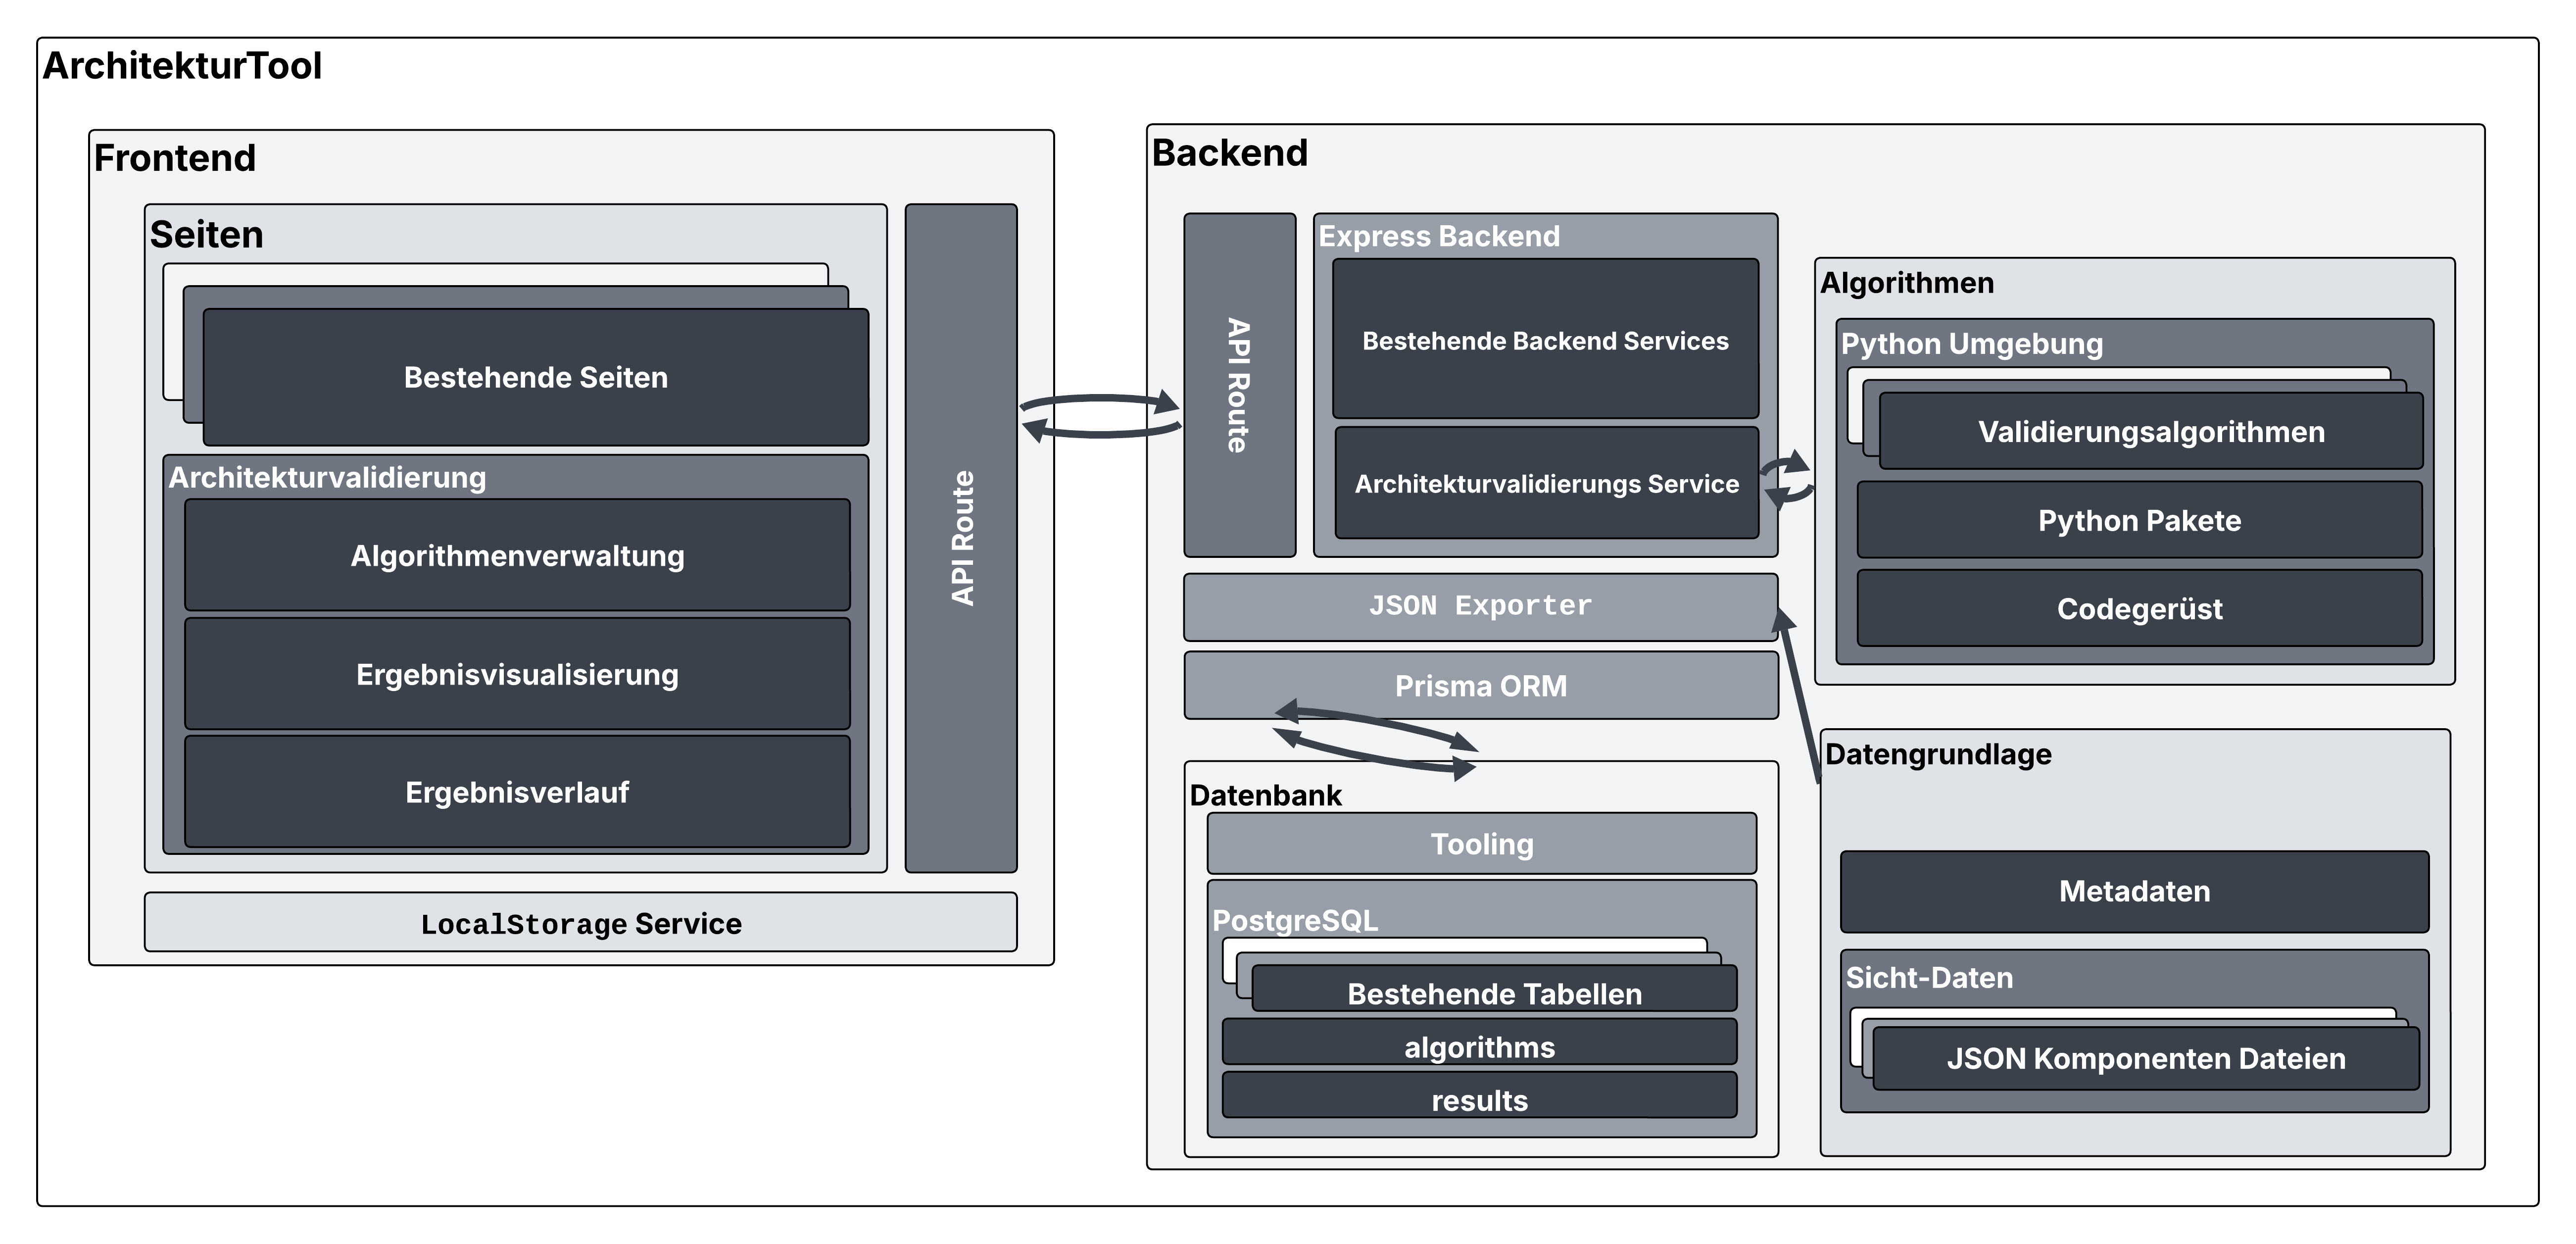
\includegraphics[width=\textwidth]{figures/04Konzeption/Blockdiagram.png}
  \caption{Blockdiagramm des ArchitekturTool's}
  \label{fig:blockdiagram}
\end{figure}


Wie im Blockdiagramm dargestellt, lässt sich die Erweiterung in vier Hauptbereiche unterteilen:

\subsection*{Algorithmenverwaltung (Frontend)}

Diese Komponente bildet die zentrale Benutzeroberfläche zur Verwaltung der Validierungsalgorithmen. Sie ermöglicht es dem Nutzer, Algorithmen hochzuladen, zu bearbeiten und zu löschen. Darüber hinaus kann über die Oberfläche ein bereits hochgeladener Algorithmus gemeinsam mit einer im Architekturtool definierten Sicht ausgewählt und ein Validierungslauf gestartet werden.

\subsection*{Ergebnisvisualisierung (Frontend)}

Diese Komponente ist ausschließlich für die Darstellung der Ergebnisse eines Validierungslaufs verantwortlich. Die empfangenen Resultate werden entsprechend ihrer Struktur aufbereitet und dem Nutzer in geeigneter Form präsentiert, je nach Definition entweder als textuelle Ausgabe (z.B. Fehlerliste) oder als grafische Darstellung (z.B. Balken- oder Netzdiagramm).Zusätzlich wird ein Verlauf der letzten zehn Validierungsergebnisse angezeigt, um Entwicklungen oder wiederkehrende Auffälligkeiten im Zeitverlauf nachvollziehbar zu machen.

\subsection*{Validierungsalgorithmus-API (Backend)}

Die \gls{api} bildet die zentrale serverseitige Schnittstelle zur Verwaltung der Validierungsalgorithmen. Sie stellt REST-Endpunkte bereit, mit denen Algorithmen hinzugefügt, ausgelesen, aktualisiert und entfernt werden können (CRUD\footnote{Create, Read, Update, Delete}-Operationen). Dadurch wird eine flexible und standardisierte Integration neuer Validierungsverfahren ermöglicht.

\subsection*{Validierung-Ausführen (Backend)}

Dieser Teil ist für die eigentliche Durchführung bzw. Berechnung zuständig. Dabei wird ein zuvor ausgewählter Validierungsalgorithmus gemeinsam mit einer spezifischen Sicht der Arhcitektur an die Funktion übergeben. Zur Ausführung wird eine isolierte Python-Umgebung genutzt, so erfolgt die Berechnung gekapselt und getrennt vom Hauptprozess des Webservers, was für Sicherheit und Stabilität sorgt.\\


Die beschriebene Systemarchitektur legt damit die technische Grundlage für die im Folgenden im detail betrachteten Komponenten und Algorithmen.

%\section{Konzept der Komponenten}

%Nachdem im vorherigen Abschnitt die übergeordnete Systemarchitektur und das Zusammenspiel der Hauptkomponenten vorgestellt wurden, befasst sich dieses Kapitel mit der detaillierten Konzeption dieser einzelnen Komponenten. Nacheinander werden der Entwurf der \gls{api}, der Algorithmenverwaltung, der Ergebnisvisualisierung sowie des Ergebnisverlaufs.

\section{API zur Algorithmenverwaltung}

Zur Verwaltung der Validierungsalgorithmen wird gemäß der Anforderung FA-1 + NFA-1 eine \gls{rest}-konforme \gls{api} zur Verfügung gestellt. Diese ermöglicht es, Algorithmen hochzuladen, zu bearbeiten, auszulesen und zu löschen. Die \gls{api} bildet die technische Grundlage für die Interaktion zwischen Frontend und Backend und wird so gestaltet, dass sie flexibel erweiterbar und robust gegenüber Fehlern ist. Die Datenbankzugriffe erfolgen über Prisma ORM, während Datei-Uploads über die Middleware \textit{Multer}\footnote{https://www.npmjs.com/package/multer} gehandhabt werden.

Die Funktionalität wird über die nachfolgend beschriebenen Endpunkte realisiert:

\subsection{CREATE - \texttt{POST /api/v2/algorithm}}

Dieser Endpunkt ermöglicht das Anbinden eines neuen Validierungsalgorithmus. Dazu wird ein Formular aus dem Frontend an das Backend übermittelt, das neben Metadaten wie Name, Beschreibung, Autor, Tags und Parametern auch die eigentlich Datei , wie in aktuellen Fall eine Python-Datei, enthält. Die Datei wird über Multer verarbeitet, wobei ein zuvor konfigurierter Speicherpfad genutzt wird. Dabei wird die hochgeladene Datei mit einem Zeitstempel versehen und im Zielverzeichnis abgespeichert, um eventuelle Namenskonflikte zu vermeiden. Eine Begrenzung der Dateigröße von 10MB schützt vor übergroßen Uploads.

Vor dem Abspeichern der Datei wird geprüft, ob bereits ein Algorithmus mit dem angegebenen Namen existiert. Ist dies der Fall, wird der Vorgang mit einem Fehlerwurf und Statuscode abgebrochen. Anschließend wird anhand der Dateiendung automatisch der Dateityp bestimmt.

Die mitgesendeten Tags und Parameter werden zunächst als JSON geparst. Abschließend wird die Datei auf dem Server abgespeichert und die Metainformationen inklusive Dateipfad über Prisma in der Datenbank festgehalten. Die Response enthalt das neu angelegte Objekt und erfolgreichen Statuscode. Uploadfehler oder fehlerhafte Eingaben werden über entsprechende Statuscodes abgefangen und mit einer passenden Fehlermeldung versendet.

\subsection{READ - \texttt{GET /api/v2/algorithms}}

Über diesen Endpunkt wird eine vollständige Liste aller, in der Datenbank abgelegten, Validierungsalgorithmen bereitgestellt. Die Daten werden mithilfe von Prisma abgefragt und als JSON an den Client(Frontend) gesendet. Dies ermöglicht die Anzeige aller verfügbaren Validierungsalgorithmen auf der Benutzeroberfläche. Im Fehlerfall wird ein entsprechender Statuscode und Fehlermeldung versendet und protokolliert.

\subsection{UPDATE - \texttt{PATCH /api/v2/algorithm/:id}}

Dieser Endpunkt dient zur Aktualisierung eines bereits bestehenden Algorithmus. Nach Erhalt der \texttt{id} aus der URL wird zunächst geprüft, ob ein entsprechender Eintrag in der Datenbank existiert. Sollte dies nicht der Fall sein, wird der Client mit einem Fehlercode informiert. Die zu aktualisierenden Daten beinhalten alle Felder, die auch bei der Erstellung der Algorithmen verfügbar waren.

Falls beim Aktualisieren eine neue Datei mitgesendet wird, wird zunächst die alte Datei aus dem Dateisystem entfernt. Anschließend wird die neue Datei gespeichert, und sowohl der neue Dateipfad als auch der aktualisierte Dateityp werden im Datenbanksatz aktualisiert. Die eigentliche Datenaktualisierung erfolgt über Prisma. Auch hier wird beim erfolgreichen Aktualisieren das Objekt als JSON zurückgegeben. Andernfalls werden auftretende Fehler, wie beispielsweise beim Dateizugriff, beim Parsen der Daten oder bei der Aktualisierung der Datenbank, abgefangen und protokolliert.

\subsection{DELETE - \texttt{DELETE /api/v2/algorithm/:id}}

Der letzte Endpunkt erlaubt das vollständige Entfernen eines Validierungsalgorithmus. Zunächst wird geprüft, ob zur übergebenen \texttt{id} ein Datensatz existiert. Ist dies nicht der Fall, wird eine Fehlermeldung zurückgegeben. Falls der Datensatz vorhanden ist, wird versucht, die zugehörige Datei aus dem Dateisystem zu löschen. Sollte die Datei nicht mehr vorhanden oder nicht zugänglich sein, wird dies in der Konsole als Warnung vermerkt und der Löschvorgang fortgesetzt.

Anschließend wird der entsprechende Eintrag in der Datenbank mithilfe von Prisma entfernt. Die Response enthält eine Bestätigung über die erfolgreiche Löschung.

\section{Grafische Benutzeroberfläche}

Um mit dem Framework zu interagieren, wird eine \gls{gui} entwickelt, die es dem Nutzer ermöglicht, Validierungsalgorithmen einfach zu verwalten, auszuführen und die Ergebnisse in passender Form einzusehen. Die \gls{gui} erweitert die zuvor beschriebene \gls{api} zur Algorithmenverwaltung um eine bedienbare Oberfläche, die sowohl technische Konfigurationen als auch visuelle Rückmeldung beinhaltet. Der Fokus liegt auf einer klaren Trennung der Bedienbereiche: zum einen die Verwaltung der Algorithmen und zum anderen die Darstellung der Validierungsergebnisse.

Die \gls{gui} folgt, wie der Rest des ArchitekturTools einem modularen Aufbau. Jeder Teilbereich, vom Hochladen über das Ausführen eines Algorithmus bis hin zur Visualisierung der Ergebnisse, ist als eigenständige Komponente realisiert. Dadurch wird die Erweiterbarkeit des Tools gewährleistet und eine klare Trennung zwischen den Funktionen ermöglicht.

Im Folgenden werden die Konzepte der Algorithmenverwaltung und Ergebnisvisualisierung genauer beschrieben.

\subsection{Algorithmenverwaltung}

Das Ziel dieser Komponente ist es, dem Nutzer eine möglichst intuitive Möglichkeit anzubieten, neue Algorithmen hochzuladen, vorhandene auszuwählen, zu bearbeiten oder zu löschen und schließlich die Validierung in Kombination mit einer ausgewählten Sicht zu starten.

Die Bedienung folgt einer funktional klar getrennten Struktur: Eine interaktive Hauptkomponente bietet die Auswahl und Steuerung, während ein Modalfenster zur Eingabe und Verwaltung der Algorithmen dient. Durch diese Aufteilung kann der Arbeitsablauf, d.h. das Verwalten und Ausführen der Algorithmen, klar gegliedert werden.

\subsubsection*{Hauptkomponente: Steuerung und Auswahl}

Innerhalb der Verwaltungs-Komponente stehen zwei Auswahlfenster zur Verfügung, eines für die bestehenden Algorithmen, das andere für die im Tool definierten Architektursichten. Nachdem beide ausgewählt wurden, kann durch einen Button ein Validierungslauf ausgeführt werden. Die Ergebnisse werden anschließend angezeigt (siehe Abschnitt~\ref{subsubsec:ergebnisvis}). Außerdem lässt sich über einen weiteren Button ein separates Modalfenster öffnen, in dem neue Algorithmen hochgeladen oder bestehende bearbeitet bzw. gelöscht werden können.

Das Konzept bezieht sich dabei auf typische Nutzungsszenarien: Im Ausgangszustand wird der Upload eines neuen Algorithmus vorgeschlagen. Sobald jedoch ein Algorithmus ausgewählt wird, wechselt der Button in den Bearbeitungsmodus. So bleibt die Bedienung dynamisch.

\subsubsection*{Modalfenster: Hochladen und Bearbeiten}

Das modale Fenster übernimmt die Erstellung und Bearbeitung einzelner Algorithmen. Neben klassischen Eingabefeldern für Name, Beschreibung, Autor, Tags und Parameter enthält das Formular auch ein integriertes Editorfeld zur Eingabe von Python-Code. Dabei wird ein Codegerüst mit bereits geladenen Packages bereitgestellt, das als Einstiegspunkt für eigene Validierungsalgorithmen dient.

Ein zentrales Konzept des Formulars ist die Wiederverwendbarkeit: Das Modal erkennt anhand übergegebener Information (ausgewählter Algorithmus), ob es sich um eine Erstellung oder eine Bearbeitung handelt, und passt den Inhalt des Formulars entsprechend an. So lassen sich bestehende Algorithmen problemlos aktualisieren bzw. vollständig entfernen. Nach Abschluss einer Aktion wird die Auswahl in der Hauptkomponente automatisch aktualisiert, sodass der Nutzer immer mit dem neuesten Datenstand arbeitet.

\subsection{(Ergebnis-)Visualisierung + Verlauf}

Nach dem Start eines Validierungslaufs besteht die zentrale Aufgabe des Tools darin, die erhaltenen Ergebnisse transparent und nutzerfreundlich darzustellen. Die grafische Visualisierungskomponente wird so entwickelt, dass verschiedene Ausgabeformate unterstützt werden und sich automatisch an den vom Algorithmus angegebenen Ergebnisdatentyp anpasst. Ergänzt wird diese Komponente durch einen Verlauf bzw. History, welcher die letzten zehn Validierungsdurchläufe archiviert und so dem Nutzer eine nachträgliche Einsicht sowie den Vergleich verschiedener Läufe ermöglicht. Zusammen bilden diese Komponenten die Grundlage für eine nachvollziehbare und stetig überprüfbare Architekturvalidierung.

\subsubsection*{Ergebnisvisuallisierung}
\label{subsubsec:ergebnisvis}

Die Ergebnisvisualisierung wird so entwickelt, dass sie auf verschiedene Ergebnistypen reagieren kann und diese übersichtlich darstellt. Je nach übermitteltem Typ wird das Ergebnis entweder als formatierter Text oder als Diagramm visualisiert. Die Auswahl der Darstellungsform erfolgt automatisch und wird innerhalb der Komponente entschieden.

Für die Visualisierung metrischer Daten wird eine eigene Hilfskomponente integriert, die verschiedene Darstellungsformen wie Linien-, Balken- oder Flächendiagramme unterstützt. Falls vom Algorithmus ein Grenzwert mitgeliefert wird, erscheint dieser als Referenzlinie im Diagramm. Datenpunkte, die diesen Grenzwert überschreiten, werden farblich markiert. Dies ermöglicht eine schnelle Interpretation und erleichtert die Bewertung der Ergebnisse.

Wie auch beim dem Modalfenster, folgt diese Komponente einem modularen und erweiterbaren Ansatz, sodass neue Ergebnisformate bei Bedarf ergänzt werden können, ohne das gesamte Framework zu verändern.

\subsubsection*{Ergebnisverlauf}
\label{subsubsec:ergebnisverlauf}


Ergänzend zu der Darstellung aktueller Ergebnisse wird eine Verlaufskomponente implementiert, welche die letzten zehn Validierungsläufe in chronologischer Reihenfolge aufführt. Jeder Eintrag enthält Eckdaten zum verwendeten Algorithmus, zur gewählten Sicht sowie den Zeitpunkt, an dem die Validierung durchgeführt wurde. Die entsprechenden Ergebnisse können aufgeklappt werden und in der selben Form wie die Hauptanzeige analysiert werden.

Das Design dieser Komponente folgt dem aufklappbaren Listenprinzip. Dadurch bleibt die Übersichtlichkeit auch bei mehreren Einträgen bestehen. Durch die Wiederverwendung des bereits beschriebenen Visualisierungskonzept, bleibt die Nutzererfahrung konsistent.

\section{Algorithmus-Ausführung}

Das Ziel dieser Komponente ist es, einen ausgewählten Validierungsalgorithmus mit einer konkreten, im ArchitekturTool bereits spezifizierten, Sicht als Eingabe auszuführen und das Ergebnis danach nutzerfreundlich bereitzustellen. Dafür wird diese Komponente so realisiert, dass sowohl die vorbereitende Datenzusammenführung als auch die Ausführung des Algorithmus sowie die Verarbeitung des Ergebnisses übernimmt.

Der Aufbau der Komponente ist so, dass sie losgelöst vom Hauptprozess des Webservers arbeitet. Dazu wird die Ausführung des Algorithmus in einem separaten Python-Prozess gestartet. Dies ermöglicht neben der Nutzung von etablierter Bibliotheken in Bezug auf die Architekturvalidierung auch verbesserte Stabilität und Sicherheit des Gesamtsystems, da potentielle Laufzeitfehler innerhalb des Skripts isoliert behandelt werden.

Zu Beginn jeder Ausführung wird ein Algorithmus und einer Sicht, über das Frontend ausgewählt und an das Backend versendet. Ausgehend von der gewählten Sicht müssen die zugehörigen Architekturkomponenten vor der Ausführung als strukturierte JSON-Dateien vorliegen. Falls dem nicht so ist, wird der Export automatisch angestoßen.

Für diesen Zweck wird eine bestehende Export-Komponente (JSON-Exporter) verwendet, die im Rahmen dieser Arbeit angepasst wurde. Diese ist dafür verantwortlich die in der Datenbank gespeicherten Komponenten, Verbindungen und Schnittstellen zu extrahieren und in ein komponentenbasiertes JSON-Format zu parsen. Dafür wird jede Komponente gemeinsam mit ihren Anforderungen, Garantien und internen Verbindungen exportiert und serverseitig in einer strukturierten Ordnerstruktur abgespeichert. Dieser wird so lange wiederverwendet, bis die zugrunde liegende Architektur verändert wird.

Nachdem alle notwendigen Dateien vorliegen, wird ein JSON-Objekt erzeugt, welches alle Komponenten der gewählten Sicht enthält. Diese Architektur wird als Eingabe an den Python-Prozess gesendet. Während der Ausführung werden sowohl Ausgabe als auch Fehlermeldungen überwacht. Nach erfolgreichem Ausführen des Skripts wird das Ergebnis interpretiert und entweder der textuelle Ausgabe oder als metrische Ausgabe zugewiesen.

Das Ergebnis wird danach gemeinsam mit weiteren Metadaten, wie Ausführungsdauer, Status und eventueller Fehlermeldung in der Datenbank abgespeichert. Diese Informationen stehen danach sowohl für die Ergebnisvisualisierung als auch für den Verlauf zur Verfügung.